\subsection{Arduino}

\par \noindent
Arduino nació en el Ivrea Interaction Design Institute como una herramienta fácil para el prototipado rápido, dirigido a estudiantes sin experiencia en electrónica y programación. Tan pronto como llegó a una comunidad más amplia, la placa Arduino comenzó a cambiar para adaptarse a las nuevas necesidades y desafíos, diferenciando su oferta de simples placas de 8 bits para productos para aplicaciones IoT, wearable, impresión 3D y entornos integrados. Todos los tableros Arduino son completamente de código abierto, lo que permite a los usuarios construirlos de forma independiente y eventualmente adaptarlos a sus necesidades particulares. El software también es de código abierto y está creciendo a través de las contribuciones de los usuarios en todo el mundo\cite{arduino-intro}.

\begin{figure}[H]
	\centering
	
\includegraphics[width=5cm, height=4cm]{arduino1.png}
	\caption{Logo Oficial de Arduino}
\end{figure}

\par
Arduino es una plataforma de electrónica de código abierto basada en hardware y software fácil de usar. Las placas Arduino pueden leer entradas (luz en un sensor, un dedo en un botón o un mensaje de Twitter) y convertirlo en una salida, activar un motor, encender un LED y publicar algo en línea. Puede decirle a su placa qué hacer enviando un conjunto de instrucciones al microcontrolador en la placa. Para hacerlo, utiliza el lenguaje de programación Arduino (basado en \textquotedblleft Wiring\textquotedblright) y el software Arduino (IDE), basado en \textquotedblleft Processing \textquotedblright\cite{arduino-intro}.

\par \noindent
Con los años, Arduino ha sido el cerebro de miles de proyectos, desde objetos cotidianos hasta complejos instrumentos científicos. Una comunidad mundial de fabricantes (estudiantes, aficionados, artistas, programadores y profesionales) se ha reunido en torno a esta plataforma de código abierto, sus contribuciones se han añadido a una increíble cantidad de conocimiento accesible que puede ser de gran ayuda para principiantes y expertos por igual\cite{arduino-intro}. A continuación, imágenes de dos de los modelos que ofrece el proyecto Arduino.

\begin{figure}[H]
	\centering
	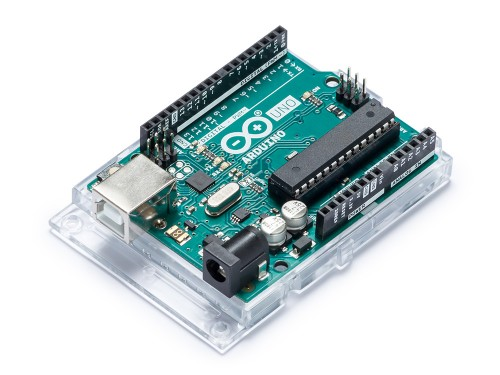
\includegraphics[width=6cm, height=5cm]{arduino2.jpg}
	\caption{Placa Arduino Uno}
\end{figure}

\begin{figure}[H]
	\centering
	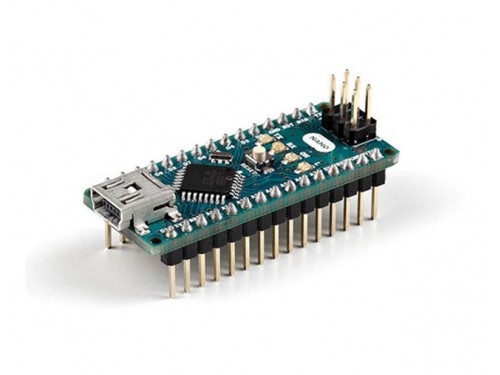
\includegraphics[width=6cm, height=5cm]{arduino3.jpg}
	\caption{Placa Arduino Nano}
\end{figure}

\subsubsection{Componentes Pasivos }

\par \noindent
Los componentes pasivos son los encargados de la conexión entre los diferentes componentes activos, asegurando la transmisión de las señales eléctricas o modificando su nivel.\cite{artofelectronics} Los componentes pasivos son:

\begin{itemize}
	\item Resistencias: Son usadas para establecer corrientes de operación y niveles de señal. Las resistencias se utilizan en los circuitos de alimentación para reducir los voltajes al disipar la potencia, medir las corrientes y descargar los capacitores después de que se desconecta la energía. Una resistencia está hecha de elementos conductores (carbono, o una película delgada de metal o carbono, o un cable de baja conductividad), con un cable o contactos en cada extremo. Las resistencias se caracterizan por su resistencia y es definido por la ley de Ohm.\cite{artofelectronics} 
	$$R = V/I$$
	Donde R es de Resistencia, V de Voltaje e I de corriente.
\end{itemize}

\begin{figure}[H]
	\centering
	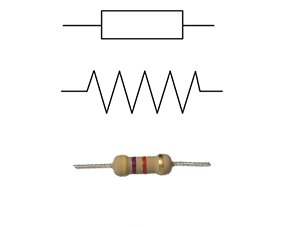
\includegraphics[width=6cm, height=4cm]{resistor1.png}
	\caption{Ejemplo de Resistor y Simbología}
\end{figure}

\begin{itemize}
	\item Capacitor: Los capacitores esencialmente almacenan energía, pero es principalmente utilizado en corriente directa para filtrar picos de voltaje provenientes de la fuente de la fuente de poder.\cite{artofelectronics} Un capacitor (el nombre antiguo era condensador) es un dispositivo que tiene dos cables que sobresalen y tiene la propiedad: 
	$$Q = CV$$
	Donde Q es carga almacenada en coulomb, C la capacitancia en faradios y V es la diferencia de potencia en voltios.
\end{itemize}

\begin{figure}[H]
	\centering
	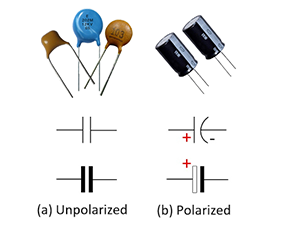
\includegraphics[width=8cm, height=6cm]{capacitor1.png}
	\caption{Ejemplo de Capacitor y Simbología}
\end{figure}

\begin{itemize}
	\item Inductor: Los inductores están estrechamente relacionados con los capacitores: la tasa de cambio de corriente en un inductor es proporcional al voltaje aplicado a través de él (para un condensador es al revés, la tasa de cambio de voltaje es proporcional a la corriente a través de él).\cite{artofelectronics} La ecuación de definición para un inductor es:
	
	$$V = L\frac{dl}{dt}$$
	
	\par \noindent
	donde $L$ se llama inductancia y se mide en henrios
	(o $mH$, $pH$, $nH$, etc.). Poniendo un voltaje constante a través de un
	inductor hace que la corriente se eleve como una rampa (en comparación con un capacitor, en el que una corriente constante causa el voltaje subir como una rampa); l $V$ a través de 1 $H$ produce una corriente que aumenta a 1 amperio por segundo.
	
	\par \noindent
	Al igual que con los capacitores, la energía invertida en el aumento de la corriente en un inductor se almacena internamente, aquí en la forma de campos magnéticos.\cite{artofelectronics}
	
\end{itemize}

\begin{figure}[H]
	\centering
	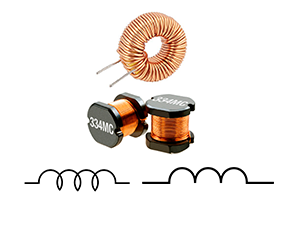
\includegraphics[width=6cm, height=4cm]{inductor1.png}
	\caption{Ejemplo de Inductor y Simbología}
\end{figure}

\par \noindent
Ya definidos los componentes que conforman los módulos de Arduino procedemos a explicar los dos módulos de comunicación que podemos encontrar en la plataforma Arduino.

\subsubsection{Módulos Arduino}

\par
Los módulos de Arduino son esencialmente placas de circuitos independientes que integran uno o múltiples circuitos integrados, sensores, pantallas LCD, componentes electrónicos y una interfaz de pines para una comunicación sencilla con la placa Arduino. Los módulos nos permiten agregar funcionalidad a nuestra placa Arduino y son como piezas de un rompecabezas donde el resultado final es el prototipo deseado.

\paragraph{Modulo Bluetooth HC-05}
El módulo HC-05 es un módulo Bluetooth SPP (Serial Port Protocol por sus siglas en inglés) fácil de usar, diseñado para la configuración de conexión en serie inalámbrica transparente. El módulo Bluetooth HC-05 se puede utilizar en una configuración maestra o esclava, lo que la convierte en una excelente solución para la comunicación inalámbrica .Este puerto en serie del módulo bluetooth es completamente calificado Bluetooth V2.0 + EDR (Enhanced Data Rate) Modulación de 3Mbps con un completo transceptor de radio de 2.4GHz y banda de base\cite{bluetooth}.

\begin{figure}[H]
	\centering
	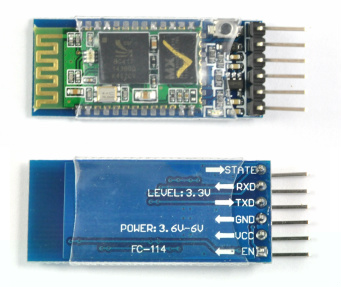
\includegraphics[width=6cm, height=4cm]{modulos1.jpg}
	\caption{Placa HC-05 Modelo ZS-040}
\end{figure}

\paragraph{Modulo Wi-Fi nRF24L01+}
El nRF24L01+ es un transceptor de 2.4GHz de un solo chip con un motor de protocolo de banda base integrado, adecuado para aplicaciones inalámbricas de muy baja potencia. El nRF24L01 + está diseñado
para el funcionamiento en la banda de frecuencia ISM mundial a 2.400 - 2.4835GHz\cite{nrf}.

\par \noindent
Para diseñar un sistema de radio con nRF24L01 +, simplemente necesita una MCU (microcontrolador) y algunos componentes externos pasivos.

\par \noindent
El motor de protocolo de banda base integrado se basa en la comunicación por paquetes
y es compatible con varios modos, desde la operación manual hasta la operación de protocolo autónomo avanzado. 
Los FIFOs internos aseguran un flujo de datos sin problemas entre la interfaz de radio y la MCU del sistema. El motor mejorado reduce el costo del sistema mediante el manejo de todas las operaciones de capa de enlace de alta velocidad\cite{nrf}.

\begin{figure}[H]
	\centering
	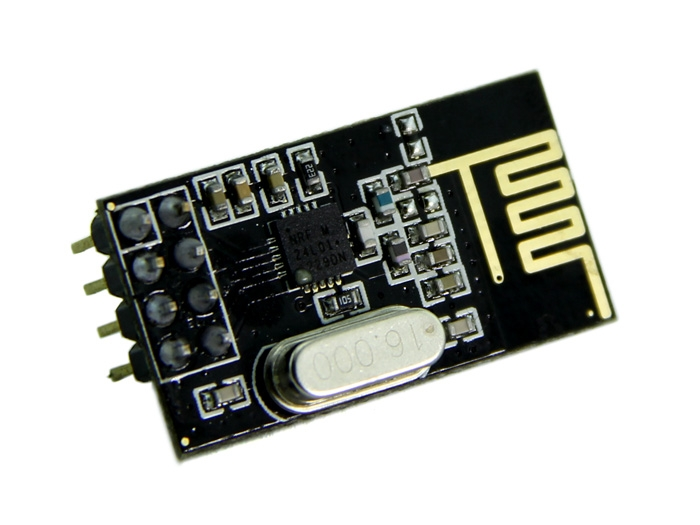
\includegraphics[width=8cm, height=6cm]{modulos2.jpg}
	\caption{Placa nRF24L01+}
\end{figure}

\par \noindent
El módulo nRF24L01+ admite una velocidad de datos de aire de 250 kbps, 1 Mbps y 2 Mbps.
La alta velocidad de datos de aire combinada con dos modos de ahorro de energía hace que el nRF24L01+ sea muy adecuado para ultra bajo
diseños de energía\cite{nrf}.

\par \noindent
El prototipo debe ser capaz de visualizar la información capturada y enviarlo a la aplicación móvil. 
Los módulos previamente mencionados son los encargados de la comunicación inalámbrica y una pantalla es la encargada de reflejar la información en tiempo real al usuario final; no obstante, primero debemos tener una lista de LCDs.

\subsubsection{Pantallas LCD}

Una pantalla LCD (Liquid Crystal Display, en inglés) es una pantalla delgada y plana formada por un número de píxeles en color o monocromos colocados delante de una fuente de luz o reflectora. A menudo se utiliza en dispositivos electrónicos de pilas, ya que utiliza cantidades muy pequeñas de energía eléctrica\cite{lcd}. Adicional las pantallas LCD deben utilizar un controlador, usualmente un circuito integrado, para poder comunicarse con las placas Arduino. 

\begin{itemize}
	\item LCM-1602: La pantalla LCM-1602 es una pantalla clásica utilizada en proyectos de Arduino. El LCM-1602 cuenta con una luz de fondo LED de color amarillo y requiere de una conexión de 5V, que puede proporcionar la mayoría de las placas Arduino. Lastimosamente solamente es capaz de visualizar 16 caracteres monocromáticos por línea, la pantalla cuenta con 2 líneas, reflejando un total de solamente 32 caracteres por líneas\cite{lcm}. Se recomienda utilizar un controlador externo para poder conectar la pantalla con Arduino; si no, se requerirían muchas más conexiones físicas para la conexión con Arduino, ver figura 2.12. Las medidas físicas de esta pantalla, hace difícil implementarla en prototipos donde el espacio se encuentra comprometido.
\end{itemize}

\begin{figure}[H]
	\centering
	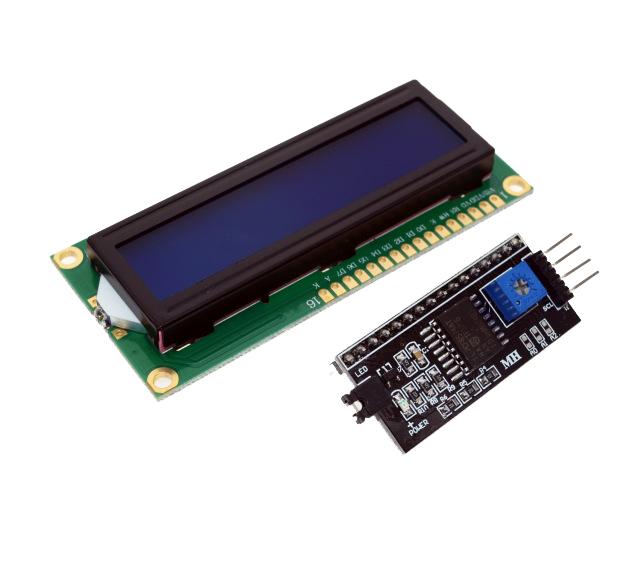
\includegraphics[width=0.5\linewidth]{lcd1.jpg}
	\caption{Pantalla LCM-1602, junto con IC para mejor integración con Arduino.}
\end{figure}

\begin{itemize}
	\item NOKIA 5110: Esta pantalla LCD es la misma utilizada por el celular Nokia 5110 o Nokia 3310, ver figura 2.13 , de allí su nombre\cite{nokia1}. 
	Sin embargo, Phillips, competencia de Nokia hace años atrás, es el fabricante del controlador de esta pantalla LCD, el PCD8544. Phillips indica que esta pantalla tiene una resolución de 48x84 pixeles; siendo esta pantalla más pequeña que el LCM-1602 pero con mayor capacidad de visualizar caracteres\cite{nokia2}. Debe ser alimentado por 3.3V exclusivamente, de ser alimentado con 5V se daña el controlador, y viene integrado con luces de fondo LED\cite{nokia2}. El único inconveniente de esta pantalla viene siendo su tamaño compacto; ya que, la visualización de la información es muy pequeña.
\end{itemize}

\begin{figure}[H]
	\centering
	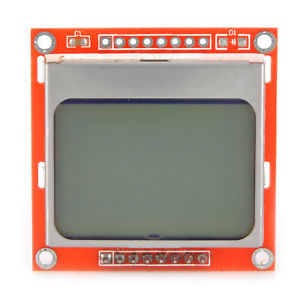
\includegraphics[width=0.4\linewidth]{lcd2.jpg}
	\caption{LCD Nokia 5110 con placa para una mejor integración con Arduino.}
\end{figure}

\begin{itemize}
	\item LCD TFT ILI9341: La pantalla LCD ILI9341 es llamado después del controlador que es utilizado para poder comunicarse con ella. Tiene versiones de 2.2, 2.4, 2.8 y 3.2 pulgadas. La pantalla ILI9341 debe ser alimentada con 5V, junto con la luz de fondo led; no obstante, el controlador utiliza una lógica de 3.3V; tiene una resolución de 240x320 pixeles y es una pantalla multicolor, excelente para dispositivo de tamaño pequeño o mediano donde una larga duración de la batería es indispensable\cite{ili9341}. 
\end{itemize}

\begin{figure}[H]
	\centering
	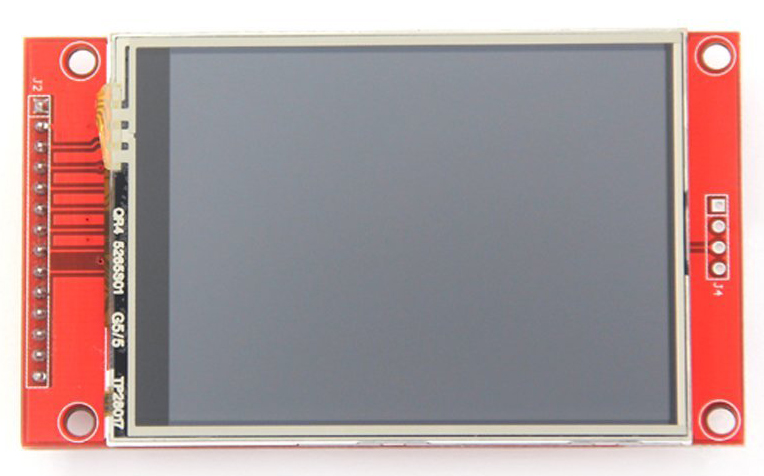
\includegraphics[width=0.5\linewidth]{lcd3.jpg}
	\caption{ILI9341 de 2.8 pulgadas con placa para mejor integración con Arduino.}
\end{figure} 

\par \noindent
Las pantallas LCD son importantes porque son el principal medio de comunicación entre el prototipo y el usuario final. Además de las pantallas LCD y los módulos de comunicación, la plataforma Arduino también soporta la implementación de sensores para poder actuar ante estímulos externos. A continuación se estarán definiendo dichos sensores

